\documentclass{article}
% translate with >> pdflatex -shell-escape <file>

% This file is used as unit test for pgfplots, copyright by Christian Feuersaenger.
% 
% See
%   http://pgfplots.sourceforge.net/pgfplots.pdf
% for pgfplots.
%
% Any required input files (for <plot table> or <plot file> or the table package) can be downloaded
% at
% http://www.ctan.org/tex-archive/graphics/pgf/contrib/pgfplots/doc/latex/
% and
% http://www.ctan.org/tex-archive/graphics/pgf/contrib/pgfplots/doc/latex/plotdata/

\usepackage{pgfplots}
\pgfplotsset{compat=1.3}

\pagestyle{empty}

\begin{document}
	\pgfplotsset{samples=10,xlabel=x,ylabel=y}
	\tikzset{domain=0:360}
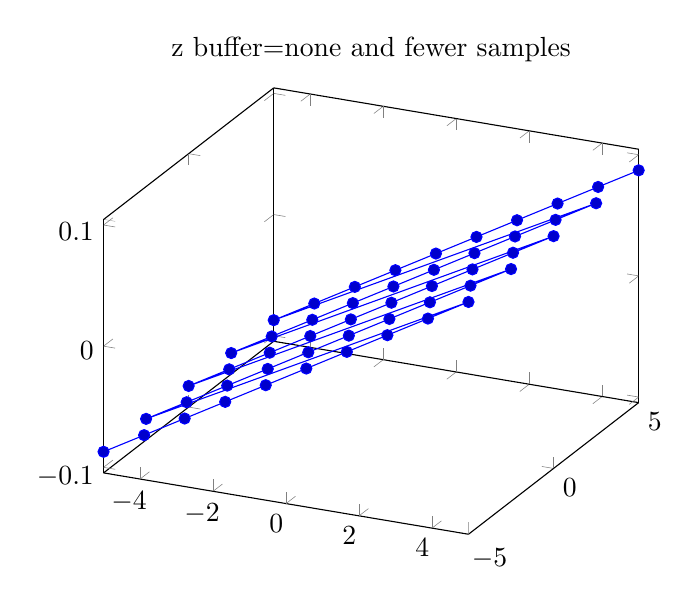
\begin{tikzpicture}
	\begin{axis}[z buffer=none,title={z buffer=none and fewer samples}]
	\addplot3+[samples=10,samples y=5] {sin(x)};
	\end{axis}
	\end{tikzpicture}
\end{document}
